\documentclass[10p]{beamer}
\usepackage[utf8]{inputenc}
\usepackage{graphicx}
\usepackage{perso}
\usepackage{animate}

\usetheme{Warsaw}
\setbeamertemplate{navigation symbols}{\insertframenumber/\inserttotalframenumber}
\setbeamerfont{block body}{size=\small}
\setbeamerfont{block body alerted}{size=\small}
\AtBeginSubsection[]
{
  \begin{frame}
  \frametitle{Sommaire}
  \tableofcontents[currentsubsection]
  \end{frame} 
}
\title{New clustering methods into a parallel code}
\author[SORIANO, AUBENEAU, DUVAL, PRIEUL, SANTINA]{SORIANO Tristan, AUBENEAU Simon, DUVAL Quentin, PRIEUL Simon, SANTINA Jeremy}
\institute{
\includegraphics[scale=0.5]{Image/logo.jpg}}
\date{\today}
\begin{document}
\begin{frame}
\maketitle
\end{frame}
\section{Introduction}
\begin{frame}
\frametitle{Clustering method}
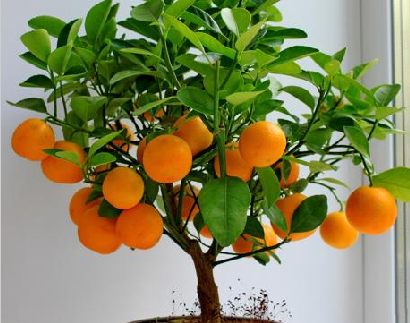
\includegraphics[width=0.5\textwidth]{Image/Oranger.png}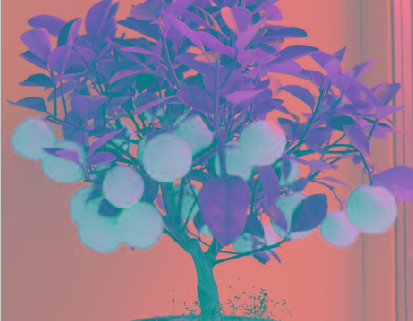
\includegraphics[width=0.5\textwidth]{Image/OrangerClust.png}
\end{frame}
\begin{frame}
\frametitle{High computational complexity}
\begin{alertblock}{Challenge}
The data used leads to computations using big dense matrices.
\end{alertblock}
\begin{center}
\only<1>{
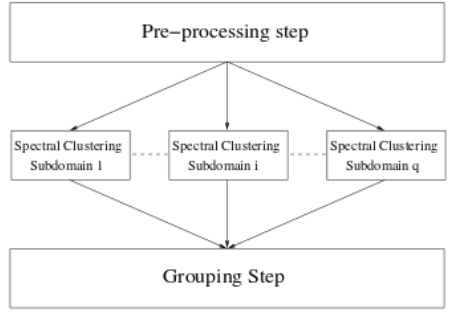
\includegraphics[width=0.5\textwidth]{Image/parallel.png}
}
\only<2>{
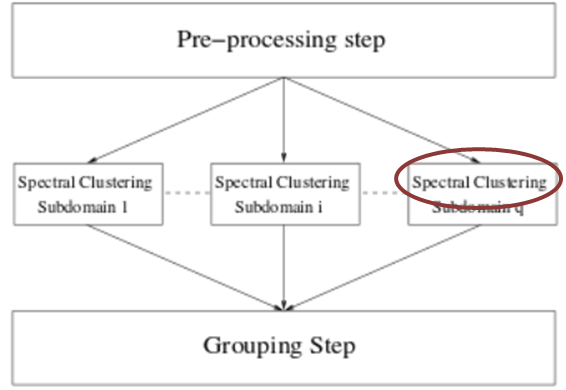
\includegraphics[width=0.5\textwidth]{Image/parallel2.png}
}
\end{center}
\end{frame}
\section{Work organisation}
\subsection{Project management}
\begin{frame}
\small
\frametitle{Development Plan}
\begin{description}
\item [Step 1] Theoretical study + Matlab new methods implementation
\item [Step 2] Code documentation + Fortran interfaces specification
\item [Step 3] Code refactoring + Fortran implementation
\item [Step 4] Validation
\end{description}
\tiny
\begin{tabular}{|l|l|l|l|}
\hline
\textbf{Risk Description} & \textbf{Probability} & \textbf{Impact} & \textbf{Action}
\\
\hline
Unsatisfied client & Light & Heavy & Specification with the client
\\
\hline
Unsuitable hardware resources & Medium & Heavy & Lighter test creation, early access request
\\
\hline
Insufficient knowledge & Heavy & Medium & Increase the time dedicated to each risky task
\\
\hline
\end{tabular}
\end{frame}
\begin{frame}
\frametitle{Team organization}
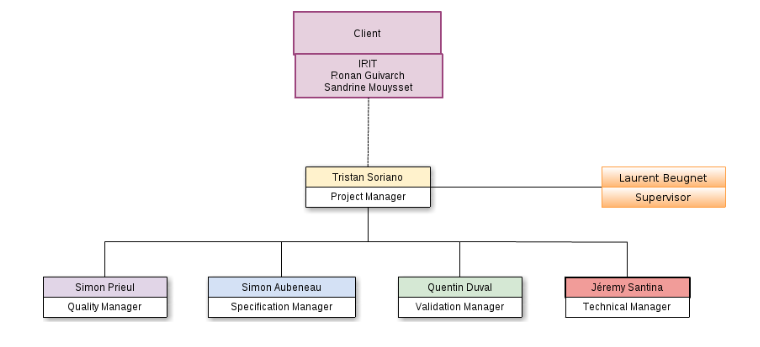
\includegraphics[width=\textwidth]{Image/organisation.png}
\end{frame}
\begin{frame}
\frametitle{Technologies}

\includegraphics[width=\textwidth]{Image/logos.png}
\end{frame}
\subsection{Starting point}
\begin{frame}
\frametitle{Environment}
\begin{block}{Source code}
A package containing source code file have been provided: functional but with a poor design.
\end{block}
\begin{block}{Configuration and setup}
\begin{itemize}
\item Libraries: MPI, Lapack and Arpack
\item F90 Compiler: GFortran
\item Configuration: Makefile
\end{itemize}
\end{block}
\end{frame}
%\begin{frame}
%\frametitle{Configuration}
%\begin{itemize}
%\item Makefile for specific environment
%\item Libraries:
%\begin{itemize}
%\item MPI
%\item Lapack
%\item Arpack
%\end{itemize}
%\item F90 compilator (gfortran, ifort…)
%\item Makefile.x has to specify the correct paths of the libraries above
%\end{itemize}
%\end{frame}
\section{Reverse engineering}
\subsection{Code refactoring}
\begin{frame}
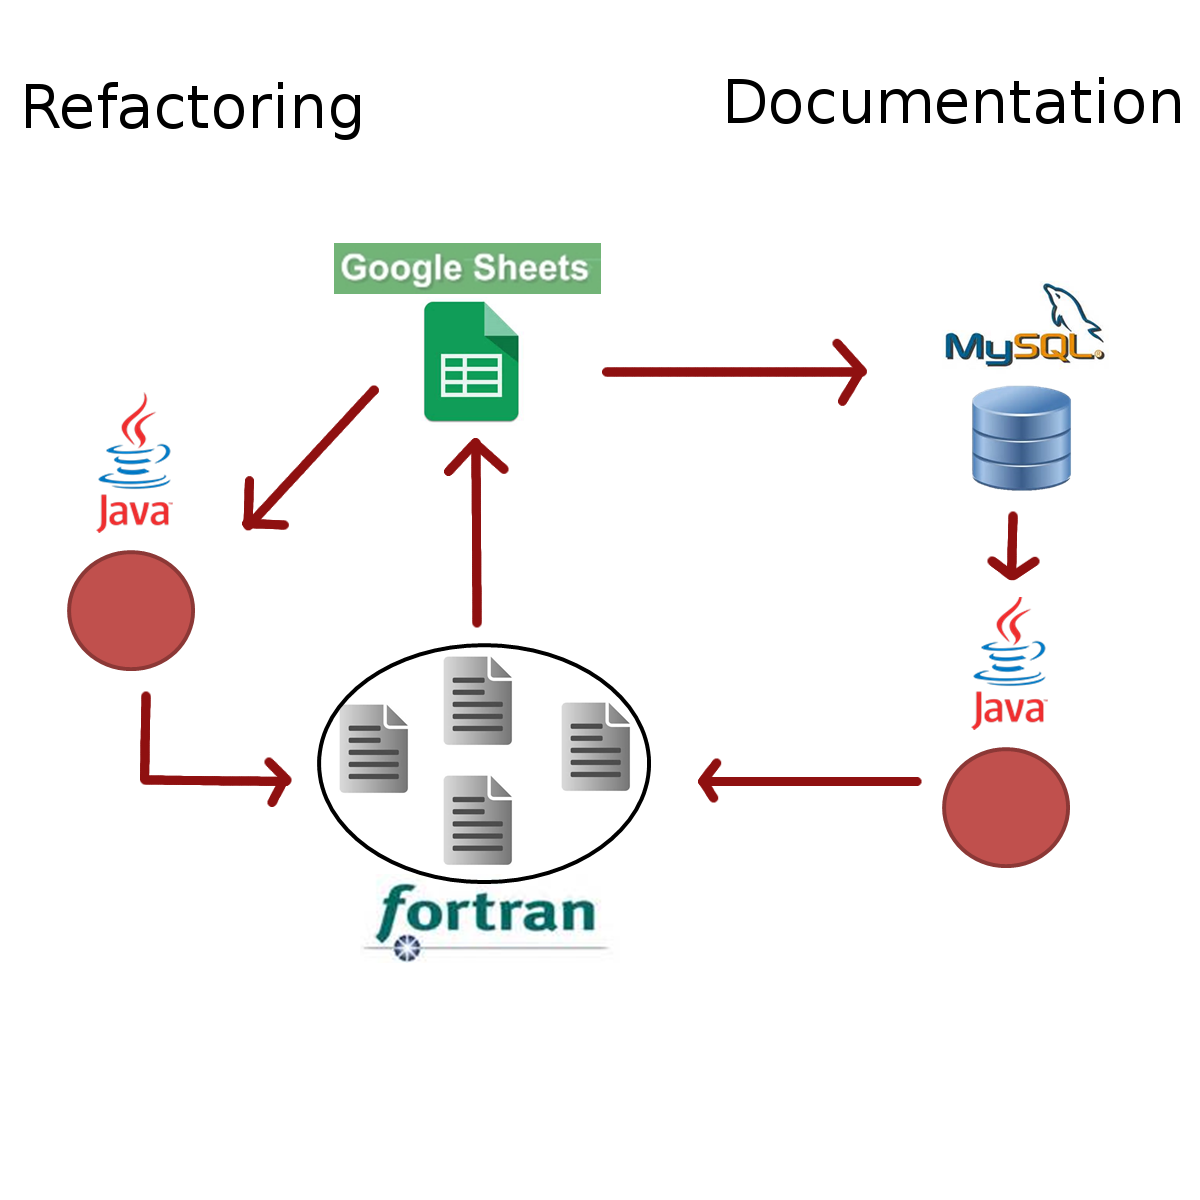
\includegraphics[scale=0.45]{Image/process.png}
\end{frame}
\begin{frame}
\frametitle{Changing source code}
\begin{block}{Purpose}
Improve software quality and portability
\end{block}
\begin{enumerate}
\item Changing the types \textit{REAL} and \textit{REAL(KIND=x)} into \textit{DOUBLE PRECISION} and \textit{INTEGER(KIND=x)} into \textit{INTEGER}
\item Changing the types \textit{CHARACTER*x} into \textit{CHARACTER (LEN=x)}
\item Changing the types of some \textit{INTEGER} variables used as boolean into \textit{LOGICAL}
\end{enumerate}
\end{frame}
\begin{frame}
\frametitle{Organising source code}
\begin{block}{Purpose}
Improve readability and maintainability of the code
\end{block}
\begin{enumerate}
\item Fortran keywords transformed in UPPERCASE
\item Removing the commented code
\item Declarations of parameters and variables at the beginning of a subroutine or program: one declaration per line, ordered by type and name
\item Removing the semicolons: only one instruction per line
\item Removing the unused variables
\end{enumerate}
\end{frame}
\begin{frame}
\frametitle{Renaming and translating}
\begin{block}{Purpose}
Improve readability and internationalization
\end{block}
\begin{enumerate}
\item Translation of the comments helping the understanding of the code
\item Rename methods: standardization (underscore to separate the different words), translation in english, better naming
\item Rename parameters of methods and local variables: standardization (underscore to separate the different words), translation in english, better naming
\item Translation of all the output console messages
\end{enumerate}
\end{frame}
\subsection{Doxygen documentation}
\begin{frame}[fragile]
\begin{block}{Produced output formats}
\begin{itemize}
\item \textit{HTML}: Documentation readable by a web browser
\item \textit{PDF}: Documentation written in LaTex to generate a PDF file
\end{itemize}
\end{block}

\frametitle{Autogeneration with Doxygen}
\begin{block}{Targets}
Description for each module, program, routine and parameters.
\end{block}

\begin{example}
\begin{lstlisting}
!> Here is a brief description of the routine.
!! @details Here is a detailed description.
!! @param[dir] param Here is the parameter description
SUBROUTINE my_routine(parameter)
\end{lstlisting}
\end{example}
\end{frame}

\begin{frame}
\frametitle{How to proceed}
\only<1>{
\begin{alertblock}{Main issues}
\begin{enumerate}
\item Renaming and reordering parameters before documenting
\item Repetitive work : 62 routines and 249 parameters
\end{enumerate}
\end{alertblock}
}
\only<1-2>{
\begin{block}{Automated comments writing}
A small software have been programmed to automatically write headers.
\end{block}
}
\only<2>{
\begin{columns}
\begin{column}{0.4\textwidth}
\begin{enumerate}
\item Classify modules, methods and parameters
\item Write descriptions in a database
\item Extract information from the database
\item Write header into the source file
\end{enumerate}
\end{column}
\begin{column}{0.6\textwidth}
\animategraphics[step,width=\columnwidth]{1}{Image/dox}{1}{5}
\end{column}
\end{columns}
}
\end{frame}
\begin{frame}[allowframebreaks]
\frametitle{Before and after}
\end{frame}
\section{Clustering algorithms}
\tableofcontents[currentsection, hideallsubsections]
\begin{frame}
\frametitle{Explanations}
\only<1>{
\begin{columns}
\begin{column}{0.4\textwidth}
\begin{itemize}
\item Spectral Clustering
\item Kernel K-Means
\item Mean Shift
\end{itemize}
\end{column}
\begin{column}{0.6\textwidth}
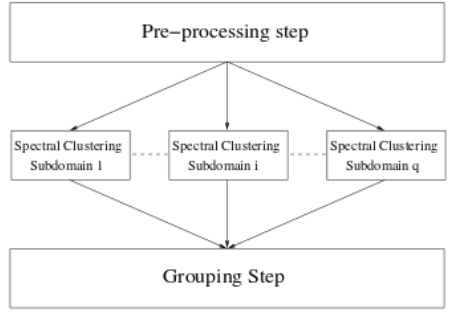
\includegraphics[width=\columnwidth]{Image/parallel.png}
\end{column}
\end{columns}
}
\only<2>{
\begin{example}
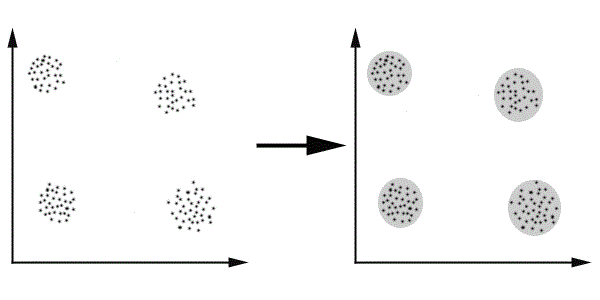
\includegraphics[width=\columnwidth]{Image/exemple.png}
\end{example}
}
\end{frame}
\subsection{Spectral Clustering}
\begin{frame}
\frametitle{Description}
\begin{block}{Main idea}
Create a weighted graph between points
\end{block}
\vfill
\begin{columns}
\begin{column}{0.6\textwidth}
\begin{itemize}
\item Each vertice weight represents the similarity between points
\item The final graph is cut on the lowest similarity vertices
\end{itemize}
\end{column}
\begin{column}{0.4\textwidth}
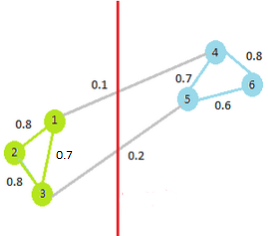
\includegraphics[width=\columnwidth, height=4cm]{Image/graph.png}
\end{column}
\end{columns}
\end{frame}
\subsection{Kernel K-Means}
\begin{frame}
\frametitle{K-Means}
\only<1>{
\begin{block}{Main idea}
Select random centers for cluster and move them until they reach centers of density.
\end{block}
\begin{columns}
\begin{column}{0.6\textwidth}
\begin{enumerate}
\item Find minimum distances to cluster centers
\item Compute density centers
\item Select new cluster centers
\item Continue until cluster centers and density centers are similar
\end{enumerate}
\end{column}
\begin{column}{0.4\textwidth}
\animategraphics[autoplay,loop,width=\columnwidth]{1}{Image/kmeans}{1}{7}
\end{column}
\end{columns}
}
\only<2>{
\begin{alertblock}{Limitation}
K-Means does not work for non-linear separations.
\end{alertblock}
\begin{columns}
\begin{column}{0.5\textwidth}

\includegraphics[width=\columnwidth]{Image/cercle.png}
\end{column}
\begin{column}{0.5\textwidth}
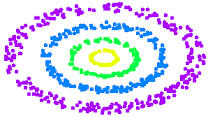
\includegraphics[width=\columnwidth]{Image/cercle2.png}
\end{column}
\end{columns}
}
\end{frame}
\begin{frame}
\frametitle{Improving K-Means}
\begin{block}{Main idea}
Using K-Means on a space with higher dimensionality to highlight separations.
\end{block}
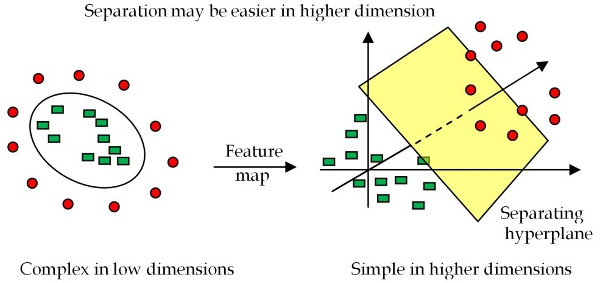
\includegraphics[width=\columnwidth]{Image/separation.jpeg}
\end{frame}
\subsection{Mean Shift}
\begin{frame}
\frametitle{Description}
\begin{block}{Main idea}
Move a window over the data set following the density gradient.
\end{block}
\begin{columns}
\begin{column}{0.6\textwidth}
\begin{enumerate}
\item Compute the mean of density in the specified window
\item Compute difference between center of the window and computed mean
\item Select the computed mean as the new center of the window
\item Restart until difference close to 0
\end{enumerate}
\end{column}
\begin{column}{0.4\textwidth}
\animategraphics[autoplay,loop,width=\columnwidth]{1}{Image/meanshift}{1}{6}
\end{column}
\end{columns}
\end{frame}
\subsection{Results}
\begin{frame}

\end{frame}
\section{Conclusion}
\begin{frame}
\end{frame}
\end{document}